\chapter{Analysis}\label{ch:analysis}

Circuit Analysis is the process of determining a circuit's behaviour from its
topology and component values. Analysis is a deterministic process, with a
variety of techniques available to a circuit designer depending on what is
already known and what is being sought.

When analysing a circuit, some characteristics are known and others are the
target of the analysis. For example,
\begin{itemize}
    \item Given a DC input voltage, what is the output voltage of a
      power supply?
    \item Given an AC input signal, what is the frequency response of a
      Low Pass Filter (LPF)?
    \item Given an AC input signal, what is the gain of a transistor
      amplifier?
\end{itemize}
This raises two natural questions:
\begin{enumerate}
    \item How many distinct kinds of analysis technique exist, in
      principle, for any given circuit?
    \item Given a set of known characteristics (AC/DC input, time/frequency
      response), which technique is the appropriate one to apply?
\end{enumerate}
To answer the first question, we build a structure that classifies every
analysis technique. Each characteristic that distinguishes one technique from
another is binary. For example, the input signal is either DC or AC; the
response is computed in either the time domain or the frequency domain; the
non-linear devices in the circuit are either retained in their full
non-linear form or replaced with a first-order (small-signal) approximation
about a bias point. The second question, which technique to apply for a
given circuit, depends on the specific problem at hand; later sections
address this with worked examples.

\section{Classification Space}

Figure~\ref{fig:analysis-classes} considers three such characteristics to
build a classification space.
\begin{enumerate}
    \item \textbf{Input Excitation:} The input is an entirely new signal of
      interest, injected at a node so that the transfer function to another
      node (acting as the output) can be computed. It is not the bias of the
      circuit. This input is either DC or AC.
      This forms the Axis of Input Excitation, the X-axis of the
      classification space.
    \item \textbf{Mathematical Representation:} The response is computed
      in either the time domain or the frequency domain. This forms the
      Axis of Mathematical Representation, the Y-axis of the classification
      space. You can flip between the time and frequency domain using a
      Fourier or Laplace Transform.
    \item \textbf{Non-Linear Device Modelling:} The non-linear devices are
      either retained in full (large-signal analysis) or linearized about
      a bias point (small-signal analysis). This forms the Axis of
      Linearity, the Z-axis of the classification space.
\end{enumerate}

\begin{figure}[H]
  \centering
  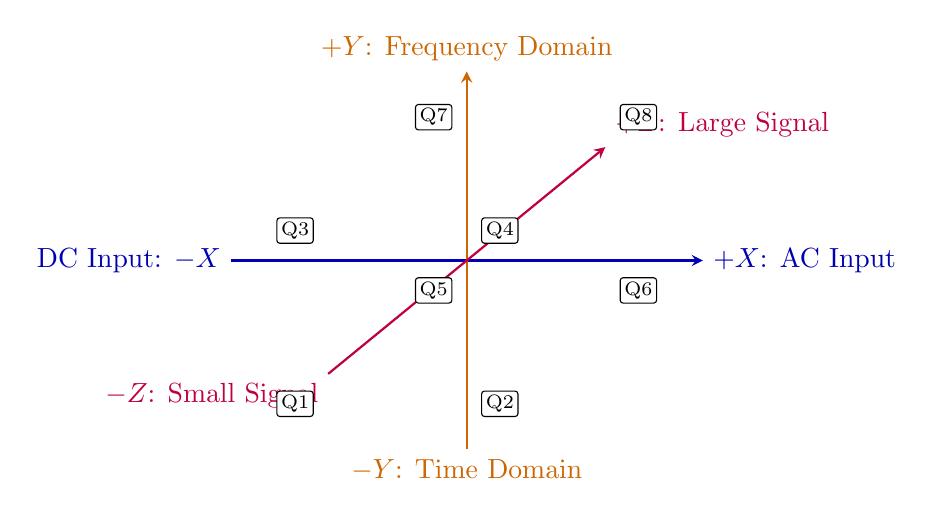
\begin{tikzpicture}[x={(1cm,0cm)}, y={(0cm,1cm)}, z={(0.55cm,0.45cm)}, >=stealth]
    \draw[->, thick, blue!70!black] (-3,0,0) -- (3,0,0) node[right] {\(+X\): AC Input};
    \node[left, blue!70!black] at (-3,0,0) {DC Input: \(-X\)};
    \draw[->, thick, orange!80!black] (0,-2.4,0) -- (0,2.4,0) node[above] {\(+Y\): Frequency Domain};
    \node[below, orange!80!black] at (0,-2.4,0) {\(-Y\): Time Domain};
    \draw[->, thick, purple] (0,0,-3.2) -- (0,0,3.2) node[above right] {\(+Z\): Large Signal};
    \node[below left, purple] at (0,0,-3.2) {\(-Z\): Small Signal};
    \foreach \x/\y/\z/\q in {-1/-1/-1/Q1, 1/-1/-1/Q2, -1/1/-1/Q3, 1/1/-1/Q4,
                             -1/-1/1/Q5, 1/-1/1/Q6, -1/1/1/Q7, 1/1/1/Q8}
      \node[draw, rounded corners=1pt, fill=white, inner sep=1.5pt, font=\scriptsize]
        at (1.3*\x, 1.1*\y, 1.6*\z) {\q};
  \end{tikzpicture}
  \caption{Classification space for analysis techniques. Octant
    \(Q_k\) has \(k - 1 = 4Z + 2Y + X\) with \(X, Y, Z \in \{0, 1\}\).}\label{fig:analysis-classes}
\end{figure}

\section{Analysis Techniques}

The resulting space has eight octants (I call them quadrants Q1 to Q8),
each corresponding to a distinct analysis technique. Let us now consider
each octant in turn, and the
analysis technique that arises from it.

\begin{itemize}
    \item \textbf{Q1: Small Signal, Time Domain, DC Input:}
      The analysis of a circuit with a DC input
      signal, where the response is computed in the time domain, and the
      non-linear devices are linearized about a bias point. In small
      signal analysis, the DC operating point is used to compute the
      linearization and is then removed from the circuit: independent DC
      voltage sources are shorted, independent DC current sources are
      opened, leaving only the incremental (perturbation) behaviour about
      that point. A DC input to this linearized circuit is therefore
      identically zero by construction. This analysis is \textbf{not useful}.
    \item \textbf{Q2: Small Signal, Time Domain, AC Input:}
      The analysis of a circuit with an AC input
      signal, where the response is computed in the time domain, and the
      non-linear devices are linearized about a bias point. It is a very
      useful technique, and is equal to the Inverse Laplace Transform of
      \textbf{Q4}.
    \item \textbf{Q3: Small Signal, Frequency Domain, DC Input:}
      It is the Laplace Transform of \textbf{Q1}, differing only in the Mathematical
      Representation used. Since \textbf{Q1} is identically zero, so is this one, by
      linearity of the transform. This analysis is \textbf{not useful}.
    \item \textbf{Q4: Small Signal, Frequency Domain, AC Input:}
      The analysis of a circuit with an AC
      input signal, where the response is computed in the frequency
      domain, and the non-linear devices are linearized about a bias
      point. It is a very useful technique. In simulators like ngspice, it
      is implemented as AC analysis.
    \item \textbf{Q5: Large Signal, Time Domain, DC Input:}
      The analysis of a circuit with a DC input
      signal, where the response is computed in the time domain, and the
      non-linear devices are retained in full. It is a very useful
      technique. In simulators like ngspice, it is implemented as DC
      analysis, OP analysis, or DC sweep analysis.
    \item \textbf{Q6: Large Signal, Time Domain, AC Input:}
      The analysis of a circuit with an AC input
      signal, where the response is computed in the time domain, and the
      non-linear devices are retained in full. It is a very useful
      technique. In simulators like ngspice, it is implemented as TRAN
      analysis.
    \item \textbf{Q7: Large Signal, Frequency Domain, DC Input:}
      It is the Laplace Transform of \textbf{Q5}, differing only in the
      Mathematical Representation used. It does contain information about
      the circuit, namely the frequency response to a DC input but since
      it is only a single frequency bin at zero, this analysis is
      \textbf{not useful}.
    \item \textbf{Q8: Large Signal, Frequency Domain, AC Input:}
      It is the Laplace Transform of \textbf{Q6},
      differing only in the Mathematical Representation used. It contains
      useful information about the circuit, namely the frequency response
      of the circuit to an AC input with one caveat: unlike
      \textbf{Q4}, the non-linear device models are not
      linearized, so superposition does not hold. The resulting spectrum
      is only valid for the specific input amplitude and waveform used to
      compute it, not a general transfer function; changing the input
      requires recomputing this octant from \textbf{Q6},
      rather than scaling the result. In simulators like ngspice, it is
      implemented as FOUR analysis.
\end{itemize}

Removing \textbf{Q1}, \textbf{Q3} and \textbf{Q7} due to lack of usefulness,
we can summarize the octants and the analysis techniques that arise
from them:
\begin{table}[H]
    \centering
    \begin{tabular}{|c|c|c|c|c|c|}\hline
      \textbf{Q} & \textbf{ZYX} & \textbf{Linearity} & \textbf{Representation} & \textbf{Input Excitation} & \textbf{SPICE} \\ \hline
      Q2 & 001 & Small Signal & Time      & AC & None \\ \hline
      Q4 & 011 & Small Signal & Frequency & AC & AC \\ \hline
      Q5 & 100 & Large Signal & Time      & DC & DC, OP, DC Sweep \\ \hline
      Q6 & 101 & Large Signal & Time      & AC & TRAN \\ \hline
      Q8 & 111 & Large Signal & Frequency & AC & FOUR \\ \hline
    \end{tabular}
    \caption{Summary of the five useful octants of analysis techniques.}\label{tab:quadrant-summary}
\end{table}

\section{Octant/Axes Dependencies}

Certain Octants and Axes are dependent on each other, and this is important to
understand when analysing circuits.
\begin{itemize}
    \item \textbf{Q2} and \textbf{Q4} depend on \textbf{Q5} to find a bias
      point to linearize the non-linear devices about.
    \item \textbf{Q6} can be computed without any knowledge of \textbf{Q5}
      but it is often useful to compute \textbf{Q5} first to find a bias
      point and use that to set initial conditions.
    \item \textbf{An AC Input} can make use of either a small signal or
      large signal device model but it is often convenient to use a small
      signal model, since it is linear and therefore easier to analyse.
      This is done below in the section on hand analysis simplifications.
\end{itemize}

\section{Hand Analysis Simplifications}

When analysing circuits by hand, it is often useful to simplify the
circuit schematic by treating various devices as either short circuits
or open circuits, depending on the input excitation AC/DC.
\begin{table}[H]
    \centering
    \begin{tabular}{|c|c|c|}\hline
      \textbf{Device}   & \textbf{DC Input} & \textbf{AC Input} \\ \hline
      DC Voltage Source & -                 & Short \\ \hline
      AC Voltage Source & Short             & -     \\ \hline
      DC Current Source & -                 & Open  \\ \hline
      AC Current Source & Open              & -     \\ \hline
      Resistor          & -                 & -     \\ \hline
      Capacitor         & Open              & Short (HF/Large C only) \\ \hline
      Inductor          & Short             & Open (HF/Large L only) \\ \hline
      Diode             & -                 & Linearize \\ \hline
      MOSFET            & -                 & Linearize \\ \hline
      BJT               & -                 & Linearize \\ \hline
      Dependent Sources & -                 & -     \\ \hline
      OpAmp             & -                 & -     \\ \hline
    \end{tabular}
    \caption{Hand analysis simplifications for various devices.}\label{tab:hand-analysis-simplifications}
\end{table}

In the above table, \textbf{-} indicates that the device is treated normally
that is without any simplification. \textbf{Short} indicates that the device
should be replaced with a short circuit and \textbf{Open} indicates that the
device should be replaced with an open circuit. \textbf{Linearize} indicates
that the full non-linear model of a device should be replaced with its
small-signal linearized model (about a bias point).

\section{Linearization (moving from +Z to -Z)}\label{sec:analysis_linearization}
Let a non-linear device be described by \(I = f(V)\). Q5 gives the bias
point \(V_Q\) and \(I_Q = f(V_Q)\). Write the total voltage as bias plus
perturbation, \(V = V_Q + V_q\) (upper case subscript for the large signal
bias, lower case for the small signal part), and expand about \(V_Q\):
\begin{align*}
  I &= f(V_Q + V_q) \\
  I &= f(V_Q) + f'(V_Q) V_q + \frac{f''(V_Q)}{2} V_q^2 + \frac{f^{\prime\prime\prime}(V_Q)}{6} V_q^3 + \cdots \\
  I - I_Q &= f'(V_Q) V_q + \frac{f''(V_Q)}{2} V_q^2 + \frac{f^{\prime\prime\prime}(V_Q)}{6} V_q^3 + \cdots \hspace{1cm} [I_Q = f(V_Q)] \\
  I_q = I - I_Q &\approx f'(V_Q) V_q = g\, V_q \hspace{1cm} [\text{keep first order term only}]
\end{align*}
The small signal conductance is \(g = f'(V_Q)\). The approximation holds
when the second order term is negligible against the first:
\begin{align*}
  \left|\frac{f''(V_Q)}{2} V_q^2\right| &\ll \left| f'(V_Q) V_q \right| \\
  \frac{|f''(V_Q)|}{2} |V_q| &\ll |f'(V_Q)| \hspace{1cm} [\text{divide by } |V_q|] \\
  |V_q| &\ll 2 \left| \frac{f'(V_Q)}{f''(V_Q)} \right| \hspace{1cm} [\text{multiply by } \tfrac{2}{|f''(V_Q)|}]
\end{align*}
For a device with more than one controlling voltage, \(I = f(V_1, V_2)\),
the same expansion gives one conductance per controlling voltage:
\begin{align*}
  I_q &\approx \left.\frac{\partial f}{\partial V_1}\right|_{Q} V_{1q}
             + \left.\frac{\partial f}{\partial V_2}\right|_{Q} V_{2q}
\end{align*}
This is where \(g_m = \partial I_D/\partial V_{GS}\) and
\(g_o = \partial I_D/\partial V_{DS}\) of a transistor come from.

\paragraph{Example (diode):} \(f(V) = I_S\left(e^{V/(nV_T)} - 1\right)\).
\begin{align*}
  f'(V_Q) &= \frac{I_S e^{V_Q/(nV_T)}}{nV_T} = \frac{I_Q + I_S}{nV_T} \hspace{1cm} [I_S e^{V_Q/(nV_T)} = I_Q + I_S] \\
  f''(V_Q) &= \frac{d}{dV}\left[\frac{I_S e^{V/(nV_T)}}{nV_T}\right]_{V_Q} = \frac{I_S e^{V_Q/(nV_T)}}{(nV_T)^2} = \frac{I_Q + I_S}{(nV_T)^2} \\
  2\left|\frac{f'(V_Q)}{f''(V_Q)}\right| &= 2 \cdot \frac{I_Q + I_S}{nV_T} \cdot \frac{(nV_T)^2}{I_Q + I_S} = 2 n V_T \\
  2 n V_T &= 2 \cdot 1 \cdot 26\,\text{mV} = 52\,\text{mV} \hspace{1cm} [n = 1,\ V_T = 26\,\text{mV}]
\end{align*}
Requiring the second order term to stay below \(10\%\) of the first:
\begin{align*}
  \frac{f''(V_Q)}{2} |V_q|^2 &\leq 0.1\, f'(V_Q) |V_q| \\
  |V_q| &\leq 0.2 \cdot \frac{f'(V_Q)}{f''(V_Q)} \hspace{1cm} [\text{divide by } \tfrac{f''(V_Q)}{2} |V_q|] \\
  |V_q| &\leq 0.2\, n V_T \hspace{1cm} \left[\frac{f'(V_Q)}{f''(V_Q)} = nV_T\right] \\
  |V_q| &\leq 0.2 \cdot 26\,\text{mV} = 5.2\,\text{mV}
\end{align*}

\section{Applying the Octants to a Block}\label{sec:analysis_workflow}
Every block in this notebook is analysed in the same order.
\begin{enumerate}
  \item \textbf{Large Signal, Time Domain, DC Input Analysis (Q5):} Set every source to its DC
    value, open capacitors, short inductors, keep full device equations.
    Write KCL at every node and solve for the bias point \((V_Q, I_Q)\).
    Check every device is in the intended region.
  \item \textbf{Linearize:} Replace every non-linear device by its small
    signal model evaluated at \((V_Q, I_Q)\)
    (Section~\ref{sec:analysis_linearization}).
  \item \textbf{Small Signal, Frequency Domain, AC Input Analysis (Q4):} Short DC voltage
    sources, open DC current sources, write KCL in admittances
    (\(G\), \(sC\), \(\frac{1}{sL}\), \(g_m\), \(g_o\)). Solve for
    \(H(s) = \frac{N(s)}{D(s)}\), \(Z_{in}\), \(Z_{out}\). Poles are roots
    of \(D(s)\), zeros are roots of \(N(s)\).
  \item \textbf{Small Signal, Time Domain, AC Input Analysis (Q2):} \(V_{out}(t) =
    \mathcal{L}^{-1}\{H(s) V_{in}(s)\}\).
  \item \textbf{Large Signal, Time Domain, AC Input Analysis (Q6):} Needed only when the input
    violates \(|V_q| \ll 2|f'/f''|\). Solve the non-linear differential
    equations (by hand when possible, otherwise TRAN).
  \item \textbf{Large Signal, Frequency Domain, AC Input Analysis (Q8):} Fourier series of the
    periodic Q6 output. Harmonics measure distortion:
    \[
      THD = \frac{\sqrt{\sum_{k=2}^{\infty} A_k^2}}{A_1}
    \]
\end{enumerate}

\paragraph{Example (Q4 to Q2):} An RC low pass has (Q4)
\(H(s) = \frac{1}{1 + sRC}\). A step of height \(V\) has
\(V_{in}(s) = \frac{V}{s}\).
\begin{align*}
  V_{out}(s) &= H(s) V_{in}(s) = \frac{V}{s(1 + sRC)} \\
  \frac{1}{s(1 + sRC)} &= \frac{a}{s} + \frac{b}{1 + sRC} \hspace{1cm} [\text{partial fractions}] \\
  1 &= a(1 + sRC) + b s \\
  s = 0 &: \hspace{0.5cm} 1 = a \\
  s = -\tfrac{1}{RC} &: \hspace{0.5cm} 1 = -\tfrac{b}{RC} \Rightarrow b = -RC \\
  V_{out}(s) &= V\left(\frac{1}{s} - \frac{RC}{1 + sRC}\right) \\
  V_{out}(s) &= V\left(\frac{1}{s} - \frac{1}{s + \frac{1}{RC}}\right) \hspace{1cm} [\text{divide top and bottom by } RC] \\
  V_{out}(t) &= V\left(1 - e^{-t/(RC)}\right) \hspace{1cm} \left[\mathcal{L}^{-1}\left\{\tfrac{1}{s}\right\} = 1,\ \mathcal{L}^{-1}\left\{\tfrac{1}{s + \frac{1}{RC}}\right\} = e^{-t/(RC)}\right] \\
  V_{out}(t) &= V\left(1 - e^{-t/T_c}\right) \hspace{1cm} [\text{Q2}, \ T_c = RC]
\end{align*}

\paragraph{Example (Q6 to Q8):} A diode biased at \(I_Q\) is driven by
\(V_q = V_p \cos(\omega t)\) with \(V_p\) not small. With
\(I_Q \gg I_S\) and \(x = \frac{V_p}{nV_T}\):
\begin{align*}
  I &= I_S\left(e^{\frac{V_Q + V_q}{nV_T}} - 1\right) \approx I_S e^{\frac{V_Q}{nV_T}} e^{\frac{V_q}{nV_T}} \hspace{1cm} [I \gg I_S] \\
  I &= I_Q e^{\frac{V_p \cos(\omega t)}{nV_T}} \hspace{1cm} \left[I_Q \approx I_S e^{\frac{V_Q}{nV_T}}\right] \\
  I &= I_Q e^{x \cos(\omega t)} \\
  I &= I_Q \left(1 + x\cos(\omega t) + \frac{x^2}{2}\cos^2(\omega t) + \frac{x^3}{6}\cos^3(\omega t) + \cdots \right) \hspace{1cm} \left[e^u = \sum_{k} \frac{u^k}{k!}\right]
\end{align*}
Using \(\cos^2\theta = \frac{1 + \cos 2\theta}{2}\) and
\(\cos^3\theta = \frac{3\cos\theta + \cos 3\theta}{4}\):
\begin{align*}
  \frac{x^2}{2}\cos^2(\omega t) &= \frac{x^2}{2} \cdot \frac{1 + \cos(2\omega t)}{2} = \frac{x^2}{4}\left(1 + \cos(2\omega t)\right) \\
  \frac{x^3}{6}\cos^3(\omega t) &= \frac{x^3}{6} \cdot \frac{3\cos(\omega t) + \cos(3\omega t)}{4} = \frac{x^3}{24}\left(3\cos(\omega t) + \cos(3\omega t)\right) \\
  I &= I_Q \left(1 + x\cos(\omega t) + \frac{x^2}{4}\left(1 + \cos(2\omega t)\right) + \frac{x^3}{24}\left(3\cos(\omega t) + \cos(3\omega t)\right) + \cdots \right) \\
  I &= I_Q \left[\left(1 + \frac{x^2}{4}\right) + \left(x + \frac{3x^3}{24}\right)\cos(\omega t) + \frac{x^2}{4}\cos(2\omega t) + \frac{x^3}{24}\cos(3\omega t) + \cdots \right]
\end{align*}
Collecting terms up to \(x^3\) (\(\frac{3x^3}{24} = \frac{x^3}{8}\)):
\begin{align*}
  A_0 &= I_Q\left(1 + \frac{x^2}{4}\right) \hspace{1cm}
  A_1 = I_Q\left(x + \frac{x^3}{8}\right) \hspace{1cm}
  A_2 = I_Q\frac{x^2}{4} \hspace{1cm}
  A_3 = I_Q\frac{x^3}{24} \\
  HD_2 &= \frac{A_2}{A_1} = \frac{\frac{x^2}{4}}{x + \frac{x^3}{8}} = \frac{x}{4\left(1 + \frac{x^2}{8}\right)} \approx \frac{x}{4} = \frac{V_p}{4nV_T} \hspace{1cm} [x^2 \ll 8] \\
  HD_3 &= \frac{A_3}{A_1} = \frac{\frac{x^3}{24}}{x + \frac{x^3}{8}} = \frac{x^2}{24\left(1 + \frac{x^2}{8}\right)} \approx \frac{x^2}{24}
\end{align*}
For example, at the \(10\%\) bound above, \(V_p = 5.2\,\text{mV}\) and
\(nV_T = 26\,\text{mV}\) give \(x = \frac{5.2}{26} = 0.2\). The second order
term is then \(\frac{x^2/2}{x} = \frac{x}{2} = 10\%\) of the first, and half
of it lands at \(2\omega\) (the other half is the DC shift):
\(HD_2 \approx \frac{0.2}{4} = 5\%\) and
\(HD_3 \approx \frac{0.2^2}{24} = \frac{0.04}{24} \approx 0.17\%\).
The bias shift \(A_0 - I_Q\) and the harmonics exist only in Q6/Q8; Q4
predicts \(A_1 = I_Q x\) and nothing else.
